\documentclass[a4paper,12pt]{article}

% ================================================== DATOS ==================================================

% Información de la materia
\newcommand{\codMateria}{TA135}
\newcommand{\nombreMateria}{Redes de Comunicaciones}
\newcommand{\cuatrimestre}{1.\textsuperscript{er} Cuatrimestre}

% Información del TP
\newcommand{\TpTitulo}{Trabajo Práctico n.° 1}
\newcommand{\fecha}{\today}
\newcommand{\curso}{Curso 1}

% Información de alumnos
\newcommand{\nombreA}{Lautaro García Vitale}
\newcommand{\padronA}{110028}
\newcommand{\emailA}{lagarciav@fi.uba.ar}

\newcommand{\nombreB}{Dante Gabriel Mele Ientile}
\newcommand{\padronB}{109494}
\newcommand{\emailB}{dmele@fi.uba.ar}

% ================================================== PAQUETES =================================================

% Codificación y lenguaje
\usepackage[utf8]{inputenc}
\usepackage[ddmmyy]{datetime}
\usepackage[language=spanish]{lipsum}
\usepackage[spanish]{datetime2}
\usepackage[T1]{fontenc}
\usepackage[spanish,es-nodecimaldot]{babel}
\usepackage[a4paper,margin=2.5cm]{geometry}
\usepackage{amsmath,amssymb,amsthm,mathtools}
\usepackage{bm}
\usepackage{physics}
\usepackage{setspace}
\usepackage{hyperref}
\usepackage{enumitem}

% Márgenes y página
\usepackage{geometry}
\usepackage{fancyhdr}
\usepackage{emptypage}
\usepackage{parskip}

% Encabezado personalizado
\pagestyle{fancy}
\fancyhf{}
\rhead{\group}
\lhead{\TpTitulo}
\cfoot{\thepage}

% Tipografía matemática
\usepackage{mathtools}
\usepackage{amssymb}
\usepackage{amsfonts}
\usepackage{amsthm}
\usepackage{yhmath}
\usepackage{dsfont}
\usepackage{esdiff}
\usepackage{xfrac}
\usepackage{siunitx}
\sisetup{per-mode=reciprocal, separate-uncertainty=true}

% Gráficos y tablas
\usepackage{graphicx}
\usepackage{float}
\usepackage{booktabs}
\usepackage{caption}
\usepackage{subcaption}
\usepackage{multirow}
\usepackage{adjustbox}
\usepackage[spanish]{babel}
\addto\captionsspanish{
  \renewcommand{\tablename}{Tabla}
}

% TikZ y gráficos avanzados
\usepackage{pgfplots}
\pgfplotsset{compat=1.18}
\usepackage{tikz}

% Código fuente y resaltado
\usepackage{minted}
\usepackage{tcolorbox}
\definecolor{codebg}{rgb}{0.95,0.95,0.95}  % Color de fondo del código
\usemintedstyle{friendly}                  % Estilo del resaltado de sintaxis
\setminted{
    linenos=true,                          % Numeración de líneas
    bgcolor=codebg,                        % Color de fondo del código
    fontsize=\footnotesize,                % Tamaño de la fuente
    frame=lines,                           % Estilo del marco
    framesep=2mm,                          % Separación del marco
    baselinestretch=1.2,                   % Espaciado entre líneas
    breaklines=true,                       % Romper líneas largas automáticamente
    encoding=utf8,                         % Codificación del archivo
    tabsize=4,                             % Tamaño de la tabulación
}

% Misceláneo
\usepackage{anyfontsize}
\usepackage{xcolor}
\usepackage{url}
\usepackage{comment}
\usepackage{multicol}
\usepackage[numbers,square]{natbib}

% Estilo de bibliografía
\bibliographystyle{IEEEtran}


% ==============================================================================================================
% ==============================================================================================================


\begin{document}

% ================================================== CARÁTULA ==================================================

\pagenumbering{arabic} % Comienza la numeración

\vspace{-1 cm} % La primera hoja tiene que tener menos espaciado

\begin{center}
  \begin{minipage}{0.8 cm}
    
\includegraphics[width=\linewidth]{img/fiuba.png}
  \end{minipage}
  \begin{minipage}{\widthof{\large{\textsc{Universidad de Buenos Aires}}}}
    \centering
    \large{\textsc{Universidad de Buenos Aires}}\\
    \large{\textsc{Facultad de Ingeniería}}\\
    \small{Año 2026 -- \cuatrimestre}
  \end{minipage}
\end{center}
\vspace{10mm}
\begin{center}
  \huge{\underline{\textsc{\nombreMateria}}} \\
  \vspace{7 pt}
  \Large{\TpTitulo \\}
   \vspace{7mm}
  \large{\curso}
\end{center}

\newcommand{\anchopadron}{\widthof{000 000}}
\begin{center}
  \begin{tabular}{l l l}
    \nombreA & \parbox{\anchopadron}{\raggedleft \padronA} & \emailA \\
    \nombreB & \parbox{\anchopadron}{\raggedleft \padronB} & \emailB
  \end{tabular}
\end{center}
\vspace{8mm}

\begin{center}
\renewcommand{\arraystretch}{1.3}
\begin{tabular}{@{}r p{0.62\textwidth}@{}}
\end{tabular}
\end{center}

\vspace{2em}
\thispagestyle{empty}

\begin{abstract}
En el presente trabajo práctico se analiza el funcionamiento de gRPC como mecanismo de comunicación distribuida sobre la arquitectura TCP/IP, integrando aspectos conceptuales y resultados experimentales obtenidos mediante Wireshark. Para ello se implementó un servicio cliente-servidor en Python a partir de una definición Protocol Buffers y se estudiaron los mensajes intercambiados entre ambas partes.

Las experiencias se desarrollaron en múltiples escenarios: comunicación local mediante la interfaz de \textit{loopback}, comunicación entre dos estaciones dentro de una misma red LAN y ensayos con carga concurrente utilizando múltiples solicitudes paralelas. Asimismo, se evaluó el comportamiento del sistema frente a retardos fijos, retardos variables (\textit{jitter}) y errores simulados del servicio.

A partir de las capturas y estadísticas obtenidas se examinan el establecimiento y cierre de conexiones TCP, el uso de HTTP/2 y sus \textit{streams}, la reutilización de \textit{sockets}, el impacto del RTT en los tiempos de respuesta, el orden relativo de consultas y respuestas concurrentes, y los códigos de estado reportados por gRPC ante condiciones normales y anómalas.

Los resultados muestran cómo gRPC aprovecha la multiplexación provista por HTTP/2 y la serialización eficiente de Protocol Buffers para sostener comunicaciones concurrentes y robustas, incluso ante variaciones de retardo y fallas inducidas.

En esta entrega, además del presente documento, se adjuntan los \textit{scritps} utilizados y las capturas obtenidas en \textit{Wireshark}. Se recomienda filtrar estas últimas mediante \texttt{tcp.port == 50051}.
\end{abstract}

\newpage   

\tableofcontents

\newpage

\section{Introducción}

Las aplicaciones modernas suelen requerir mecanismos de comunicación eficientes, confiables y escalables para intercambiar información entre procesos distribuidos. En ese contexto, gRPC surge como una alternativa ampliamente adoptada para la implementación de servicios remotos de alto rendimiento, al combinar el transporte provisto por TCP, las capacidades de multiplexación de HTTP/2 y la serialización compacta de Protocol Buffers.

El objetivo de este trabajo es estudiar, desde una perspectiva práctica, cómo se materializan dichos mecanismos en una implementación real. Para ello se desarrollaron experiencias controladas con cliente y servidor gRPC en Python, complementadas con capturas de tráfico mediante Wireshark. El análisis incluye tanto el comportamiento básico de una consulta RPC como situaciones más exigentes, con múltiples solicitudes concurrentes, retardos artificiales y respuestas con error.

A través de estos ensayos se busca relacionar los conceptos teóricos de las capas de transporte y aplicación con evidencia experimental, permitiendo comprender de qué manera los parámetros de red y las decisiones de diseño del protocolo influyen sobre el desempeño observado.

\section{\textit{Google Remote Procedure Calls} (gRPC)}

\textit{Google Remote Procedure Calls} (\textbf{gRPC}) es un marco de trabajo de código abierto orientado a la implementación de llamadas a procedimientos remotos (RPC), diseñado para facilitar la comunicación eficiente entre aplicaciones distribuidas. Permite que un cliente invoque métodos ubicados en un servidor remoto como si fueran funciones locales, abstrayendo gran parte de la complejidad asociada al intercambio de mensajes en red.

Además, gRPC se apoya en \textbf{HTTP/2} como protocolo de aplicación subyacente, lo que le permite aprovechar características modernas como la multiplexación de múltiples flujos de datos sobre una única conexión, compresión de cabeceras y comunicación bidireccional persistente. Dentro de HTTP/2, cada intercambio se organiza mediante un \textbf{\textit{stream}}, entendido como un flujo independiente de datos dentro de una conexión multiplexada.

En la capa de transporte, la comunicación se establece típicamente sobre \textbf{TCP} (\textit{Transmission Control Protocol}), el cual proporciona un canal confiable, orientado a conexión y de tipo \textit{full-duplex}, garantizando la entrega ordenada de los segmentos transmitidos.

Uno de los elementos centrales de gRPC es el \textbf{\textit{channel}}, que representa una conexión lógica entre cliente y servidor. Sobre un mismo \textit{channel} pueden coexistir múltiples invocaciones RPC reutilizando la misma conexión física, mejorando la eficiencia y reduciendo la sobrecarga de establecimiento de sesiones.

Para la definición de interfaces y estructuras de datos, gRPC utiliza \textbf{\textit{Protocol Buffers}}, un mecanismo de serialización binaria compacto y eficiente. Los servicios, métodos y mensajes se describen en archivos con extensión \texttt{.proto}, a partir de los cuales se genera automáticamente código cliente y servidor en diversos lenguajes de programación.

Asimismo, gRPC soporta distintos modelos de interacción. Entre ellos se encuentra la \textbf{\textit{Unary} RPC}, en la cual el cliente envía una única solicitud y recibe una única respuesta. También se dispone de \textbf{\textit{Bidirectional Streaming} RPC}, modalidad en la que cliente y servidor pueden enviarse múltiples mensajes de forma simultánea e independiente, sin necesidad de respetar un orden estricto entre emisiones.

Cada invocación RPC finaliza con un \textbf{\textit{StatusCode}}, código que informa si la operación fue exitosa o si ocurrió algún tipo de error (por ejemplo, recurso inexistente, \textit{timeout} o permisos insuficientes). Además, gRPC permite definir un \textbf{\textit{deadline}}, es decir, un límite máximo de tiempo para completar una llamada remota. Si dicho tiempo se excede, la operación se cancela automáticamente, evitando bloqueos indefinidos y mejorando la robustez del sistema distribuido.




\section{Comunicación gRPC capturada en Wireshark}

Con el objetivo de estudiar el funcionamiento de gRPC sobre la pila de protocolos TCP/IP, se realizaron capturas con Wireshark en dos escenarios distintos: primero con cliente y servidor ejecutándose en una misma estación, y luego en dos estaciones diferentes dentro de una misma red LAN. A partir de dichas capturas se analizan la interfaz utilizada, la versión de IP empleada, los puertos involucrados, el establecimiento y cierre de conexión TCP, el uso de \textit{streams} HTTP/2 y el impacto temporal de utilizar \textit{loopback} frente a una red física.

\subsection{Escenario 1: cliente y servidor en la misma estación}

\begin{figure}[H]
\centering
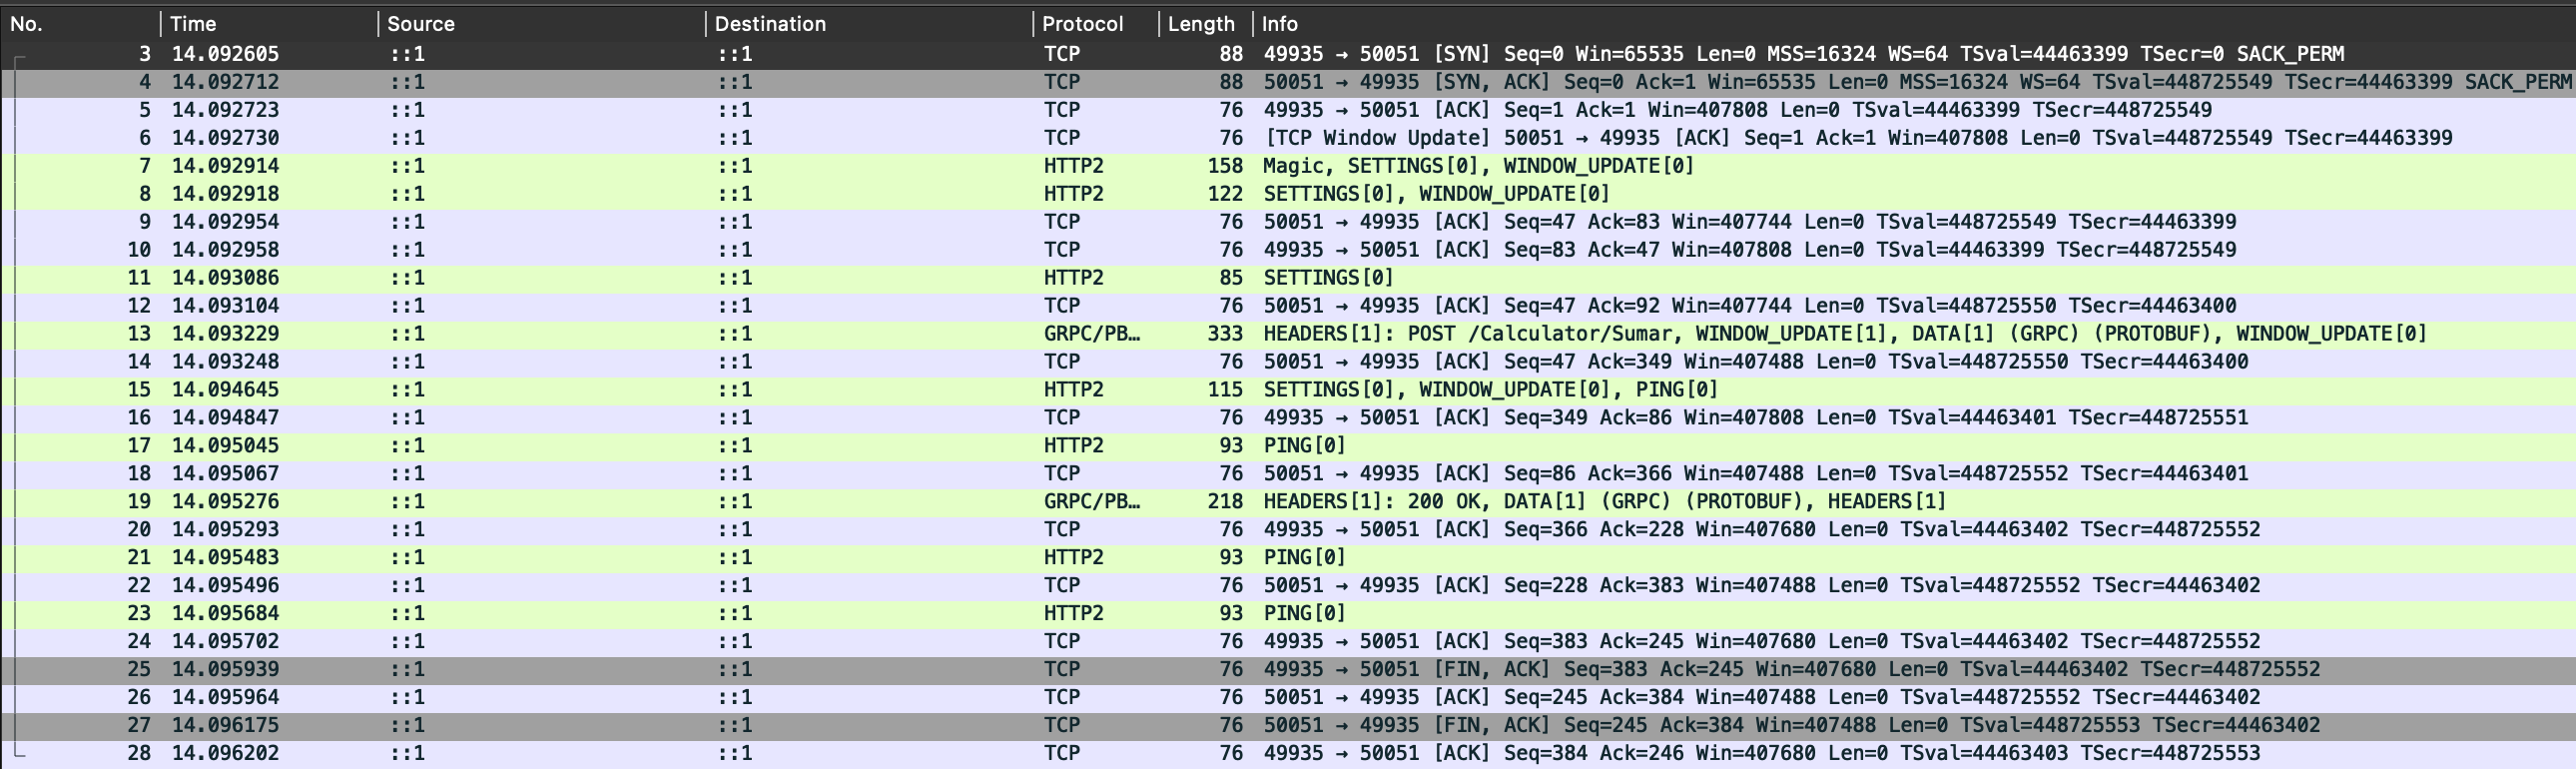
\includegraphics[width=\linewidth]{img/wireshark.png}
\caption{Captura Wireshark de la comunicación gRPC en una misma estación.}
\label{fig:grpc_local}
\end{figure}

Cuando cliente y servidor se ejecutan en la misma computadora, la comunicación aparece en la interfaz \texttt{lo0}, correspondiente al dispositivo de \textit{loopback} del sistema operativo. Esto se debe a que los paquetes nunca abandonan la máquina, sino que son encaminados internamente por la pila de red. Por esa razón, no intervienen interfaces físicas como Ethernet o Wi-Fi.

Si se desea forzar el uso de una interfaz física determinada, basta con que el cliente se conecte a la dirección IP real de la placa de red correspondiente en lugar de utilizar \texttt{localhost}. Por ejemplo, usando la IP local de Wi-Fi o Ethernet, el sistema operativo enruta el tráfico por dicha interfaz.

\subsubsection{Versión de IP utilizada}

En la captura de la Figura \ref{fig:grpc_local} se observa que las direcciones origen y destino corresponden a \texttt{::1}, es decir, la dirección de \textit{loopback} de IPv6. Por lo tanto, la comunicación se realizó mediante IPv6.

Es posible forzar IPv4 utilizando \texttt{127.0.0.1}, mientras que utilizando \texttt{::1} o resolviendo \texttt{localhost} con preferencia IPv6 se empleará IPv6. La validación experimental surge directamente de las direcciones mostradas por Wireshark.

\subsubsection{Puerto de escucha del servidor}

El primer segmento TCP muestra una conexión desde un puerto efímero del cliente hacia el puerto \texttt{50051}, por lo que se concluye que el servidor escucha en dicho puerto. Este puerto no corresponde a una asignación oficial estándar de IANA para gRPC, pero es ampliamente utilizado por convención en ejemplos y aplicaciones de prueba.

\subsubsection{Ejecución simultánea de dos servidores}

Si el servidor ya se encuentra ejecutándose y se intenta lanzar una segunda instancia usando el mismo puerto, el sistema operativo rechaza la operación con un error del tipo \texttt{Failed to add port to server: No address added out of total 1 resolved for \\ '[::]:50051'}. En ese caso no se establece una nueva sesión TCP válida, por lo que no aparece tráfico gRPC adicional significativo en la captura.

\subsubsection{Consulta simple: paquetes intercambiados}

Durante una única consulta entre cliente y servidor se distinguen tres etapas principales:

\begin{itemize}
    \item \textbf{Establecimiento de conexión TCP (3-way handshake):} segmentos \texttt{[SYN]}, \texttt{[SYN,ACK]} y \texttt{[ACK]}, observados en los paquetes 3, 4 y 5.
    
    \item \textbf{Intercambio de datos de aplicación:} luego del establecimiento se intercambian tramas correspondientes a HTTP/2 y gRPC, entre ellas mensajes \texttt{SETTINGS}, \texttt{WINDOW\_UPDATE}, \texttt{HEADERS}, \texttt{DATA} y \texttt{PING}. La invocación RPC se observa como:
    
\begin{verbatim}
POST /Calculator/Sumar
\end{verbatim}

seguida por la respuesta del servidor:

\begin{verbatim}
200 OK
\end{verbatim}

    \item \textbf{Cierre ordenado de conexión TCP:} segmentos \texttt{[FIN,ACK]}, \texttt{[ACK]}, \texttt{[FIN,ACK]} y \texttt{[ACK]}, correspondientes a los paquetes 25, 26, 27 y 28.
\end{itemize}

Tomando como inicio el primer segmento del handshake (paquete 3) y como fin el último \texttt{ACK} del cierre (paquete 28), se contabilizan 26 tramas capturadas en total. La mayoría de ellas cuentan con \texttt{Len=0}, lo que implica que no hay datos útiles enviados, por ejemplo, tratándose de segmentos de confirmación.

El tiempo total de la sesión resulta:

\[
14.096202 \text{ s} - 14.092605 \text{ s} = 0.003597 \text{ s} = 3.597 \text{ ms}
\]

\subsubsection{Opciones TCP negociadas}

Durante el establecimiento de conexión se observan las siguientes opciones TCP negociadas:

\begin{itemize}
    \item \texttt{MSS = 16324}
    \item \texttt{Window Scale = 64}
    \item \texttt{SACK\_PERM} 
    \item \texttt{TSval} y \texttt{TSecr} 
\end{itemize}

siendo \texttt{SACK\_PERM} la opción que habilita la retransmisión únicamente de los segmentos perdidos. Además, \texttt{TSval} (\textit{value}) y \texttt{TSecr} (\textit{echo reply}) son TCP \textit{timestamps} que permiten un cálculo preciso del RTT en el entorno local. 

El tamaño inicial de ventana anunciado por el cliente en el segmento SYN fue:

\[
\texttt{Win = 65535 \ bytes}
\]

Luego de aplicar el factor de escalado negociado, la ventana efectiva pasa a ser mayor, como se observa en los paquetes siguientes.

\subsubsection{Persistencia de la conexión}

En esta ejecución la conexión no permaneció abierta luego de finalizar la consulta RPC, sino que fue cerrada inmediatamente después de enviada la respuesta. Por lo tanto, no se utilizó persistencia para múltiples invocaciones sucesivas.

El primer segmento de cierre es el paquete 25:

\[
49935 \rightarrow 50051 \quad \texttt{[FIN,ACK]}
\]

por lo que el cierre fue iniciado por el cliente.

\subsubsection{Streams HTTP/2 y legibilidad}

En la captura se distinguen dos identificadores de stream HTTP/2:

\begin{itemize}
    \item \textbf{Stream 0:} reservado para control de conexión. Allí aparecen mensajes \texttt{SETTINGS}, \texttt{PING} y \texttt{WINDOW\_UPDATE}.
    
    \item \textbf{Stream 1:} utilizado para la llamada RPC principal, visible en mensajes \texttt{HEADERS[1]} y \texttt{DATA[1]}.
\end{itemize}

Parte de la información de aplicación es legible en Wireshark, por ejemplo:

\begin{itemize}
    \item \texttt{POST /Calculator/Sumar}
    \item \texttt{200 OK}
\end{itemize}

Sin embargo, la carga útil transportada por gRPC aparece serializada como:

\begin{verbatim}
DATA (GRPC) (PROTOBUF)
\end{verbatim}

por lo que no se visualiza directamente como texto plano.

A diferencia de HTTP/1.1, donde suelen observarse líneas explícitas en texto plano (ASCII) como:

\begin{verbatim}
GET /sumar?a=10&b=5 HTTP/1.1
POST /api/calculator/sumar HTTP/1.1
\end{verbatim}

gRPC utiliza HTTP/2 con tramas binarias multiplexadas y compresión de cabeceras, enviando \textit{payloads} binarios, reduciendo la legibilidad directa de la captura pero mejorando la eficiencia del transporte.


\subsection{Escenario 2: cliente y servidor en dos estaciones de la misma LAN}

\begin{figure}[H]
\centering
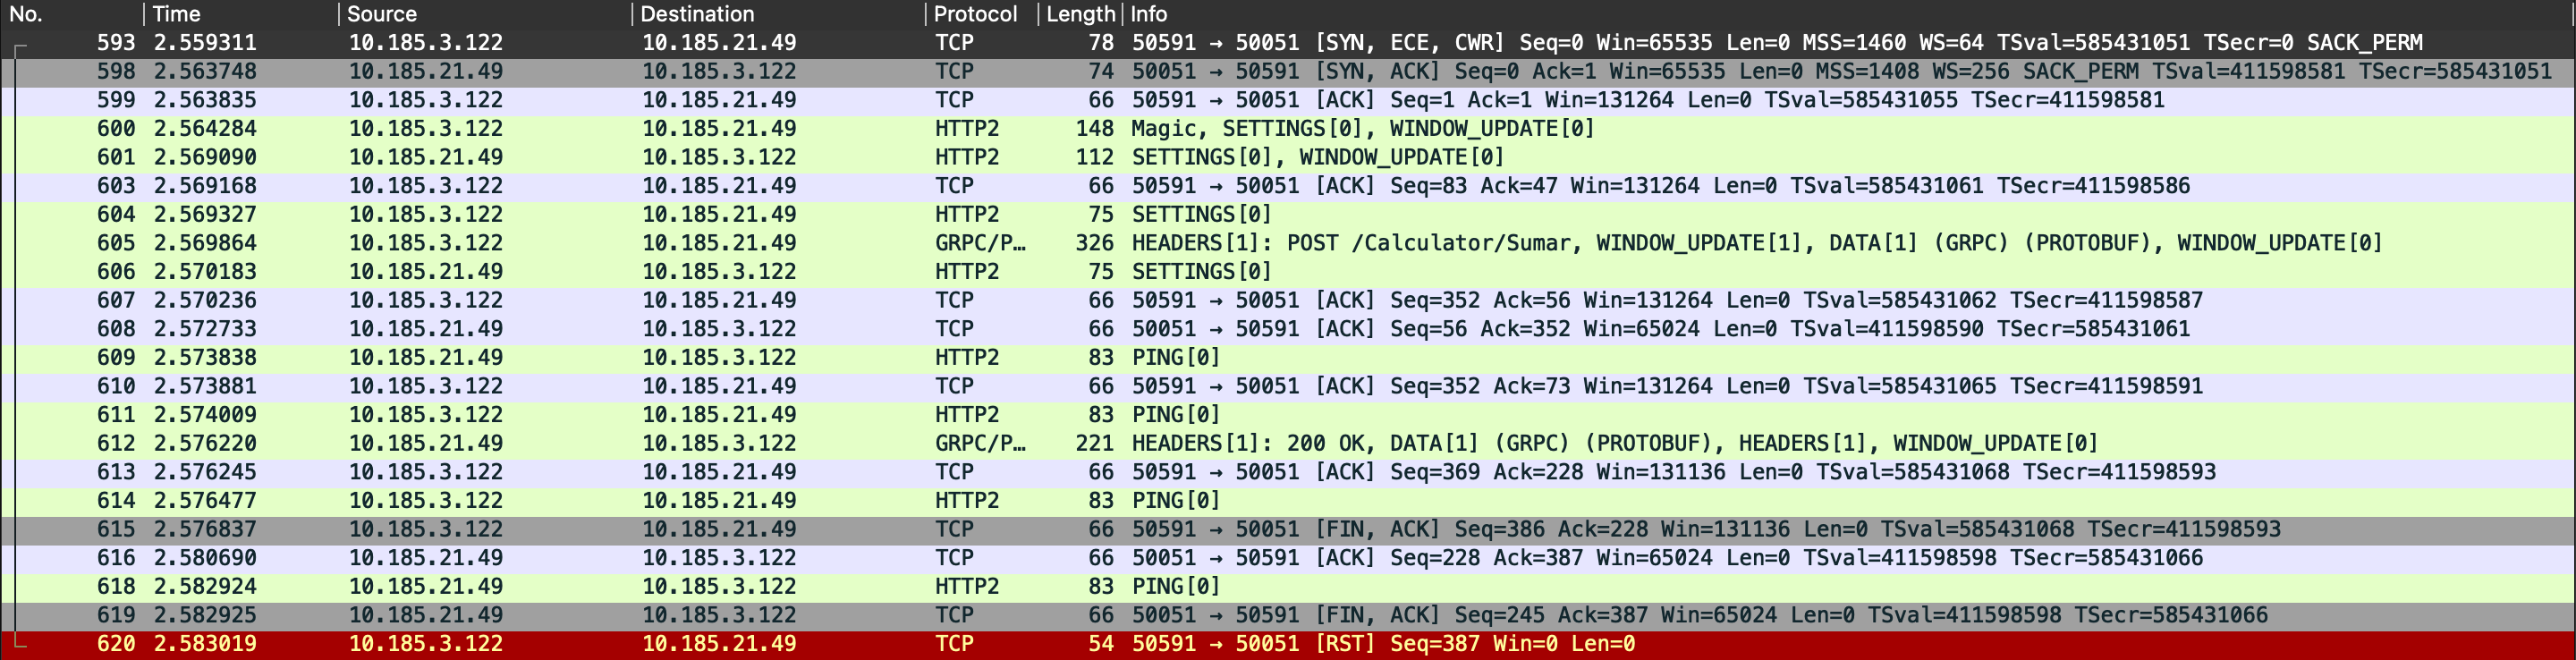
\includegraphics[width=\linewidth]{img/punto4.png}
\caption{Captura Wireshark de una consulta gRPC entre dos estaciones distintas en la LAN.}
\label{fig:grpc_lan}
\end{figure}

En este segundo escenario, cliente y servidor se ejecutan en equipos distintos conectados a la misma red local. Las direcciones IP observadas son \texttt{10.185.3.122} y \texttt{10.185.21.49}, por lo que el tráfico ya no circula por la interfaz de \textit{loopback}, sino a través de una interfaz física Ethernet o Wi-Fi.

\subsubsection{Consulta simple y tiempos medidos}

Se repite la misma prueba de una consulta gRPC simple. En la captura se distinguen nuevamente tres etapas:

\begin{itemize}
    \item \textbf{Establecimiento de conexión TCP (3-way handshake):} segmentos \texttt{[SYN]}, \texttt{[SYN,ACK]} y \texttt{[ACK]}, correspondientes a los paquetes 593, 598 y 599.
    
    \item \textbf{Intercambio de datos:} tramas HTTP/2 y gRPC con mensajes \texttt{SETTINGS}, \texttt{WINDOW\_UPDATE}, \texttt{HEADERS}, \texttt{DATA} y \texttt{PING}. La solicitud aparece como:
    
\begin{verbatim}
POST /Calculator/Sumar
\end{verbatim}

y la respuesta del servidor como:

\begin{verbatim}
200 OK
\end{verbatim}

    \item \textbf{Cierre de conexión:} el cliente inicia el cierre con un segmento \texttt{[FIN,ACK]} (paquete 615), el servidor responde con \texttt{[ACK]} (paquete 616), luego transmite \texttt{[FIN,ACK]} (paquete 619) y finalmente el cliente responde con un segmento \texttt{[RST]} (paquete 620), en lugar del \texttt{ACK} final habitual.
\end{itemize}

Tomando como referencia el primer segmento del establecimiento y el último paquete observado, el tiempo total de la sesión es:

\[
2.583019 \text{ s} - 2.559311 \text{ s} = 0.023708 \text{ s} = 23.708 \text{ ms}
\]

Comparado con el escenario local:

\[
23.708 \text{ ms} > 3.597 \text{ ms}
\]

se evidencia un incremento significativo de latencia.

\subsubsection{Origen de la diferencia temporal}

En la interfaz de \textit{loopback} sólo intervienen:

\begin{itemize}
    \item procesamiento del sistema operativo,
    \item copias en memoria,
    \item cambios de contexto entre procesos,
    \item ejecución local de cliente y servidor.
\end{itemize}

En una red LAN real se agregan además:

\begin{itemize}
    \item acceso al medio físico,
    \item transmisión por cable o Wi-Fi,
    \item retardo de propagación,
    \item procesamiento en \textit{switches} o puntos de acceso,
    \item colas de espera y \textit{buffering},
    \item posibles retransmisiones de capa física.
\end{itemize}

Por ello, la latencia total resulta mayor.

\subsubsection{Impacto en el RTT y negociación TCP}

En el escenario local, el RTT es extremadamente pequeño, permitiendo una negociación TCP casi instantánea. En la LAN el RTT aumenta debido al trayecto real entre ambos hosts, lo cual repercute en:

\begin{itemize}
    \item temporizadores iniciales TCP,
    \item cálculo del RTO,
    \item crecimiento inicial de la ventana de congestión,
    \item tiempo de establecimiento de sesión.
\end{itemize}

\subsubsection{Parámetros observados}

Durante el establecimiento de conexión se observan las siguientes opciones TCP:

\begin{itemize}
    \item \texttt{MSS = 1460}
    \item \texttt{Window Scale = 64} (cliente)
    \item \texttt{Window Scale = 256} (servidor)
    \item \texttt{SACK Permitted}
    \item \texttt{TCP Timestamps}
\end{itemize}

El valor de MSS es consistente con una MTU Ethernet típica de 1500 bytes, a diferencia del valor considerablemente mayor observado en la interfaz de \textit{loopback}.

\subsection{Comparación de resultados}

La comunicación gRPC sobre una misma estación utiliza la interfaz de \textit{loopback} y presenta tiempos mínimos debido a la ausencia de tránsito físico. En cambio, al ejecutar cliente y servidor en dos equipos distintos dentro de una misma LAN, aparecen retardos propios de la red y aumenta el RTT, impactando tanto en el tiempo total de consulta como en el comportamiento dinámico de TCP.

Asimismo, en ambos escenarios se verifica que gRPC opera sobre TCP y HTTP/2, utilizando \textit{streams} multiplexados y cargas serializadas mediante Protocol Buffers.

\section{Comunicación gRPC con alteraciones}
En esta sección utilizaremos los \textit{scripts} \texttt{server\_delay.py} y \texttt{client\_parallel.py} provistos por la cátedra para simular un \textit{delay} medio y \textit{jitter} entre consultas y respuestas y errores de servicio en el primero; \texttt{N} peticiones gRPC en el segundo.

\subsection{Escenario 1: \texttt{delay = 0}, \texttt{jitter = 0}, \texttt{errores = 0}, \texttt{N = 100} }

HTTP/2 utiliza la siguiente convención para asignar \textit{stream} ID:
\begin{itemize}
    \item \texttt{[0]}: Reservado para controles de conexión (tal y como se indicó en la sección anterior);
    \item \texttt{[impares]}: Reservado para el cliente;
    \item \texttt{[pares]}: Reservado para el servidor. 
\end{itemize}
Es por esto que se observa que, luego del \textit{stream} 0 y dado que el servidor no envía datos, los \textit{streams} IDs de esta comunicación serán 1, 3, 5, ..., 199.

Esta convención permite la multiplexación, posibilitando que el cliente envíe \texttt{N} peticiones simultaneas en una misma conexión TCP con un stream ID impar ---el mismo que utilizará el servidor para responder---.

El RTT medio obtenido en esta comunicación es 34.613 ms y su desvío estándar resultó 12.824 ms. 

En la Figura \ref{fig:5_a} se observan las primeras 26 tramas de esta comunicación. Nótese que en la trama n.° 549 el cliente envía la primera solicitud de suma ``\texttt{HEADERS[1]: POST / Calculator ...}'' y en la 563 el servidor responde ``\texttt{HEADERS[1]: 200 OK, DATA[1] ...}''. Además, nótese que en la trama 551, se envían 23 \textit{streams} en conjunto (\texttt{ID [3], ... ID [49]}). 

Este comportamiento permite observar la característica concurrente de las transacciones, en donde el cliente no espera a recibir el ``\texttt{200 OK}'' del servidor para enviar los paquetes.

\begin{figure}[H]
\centering
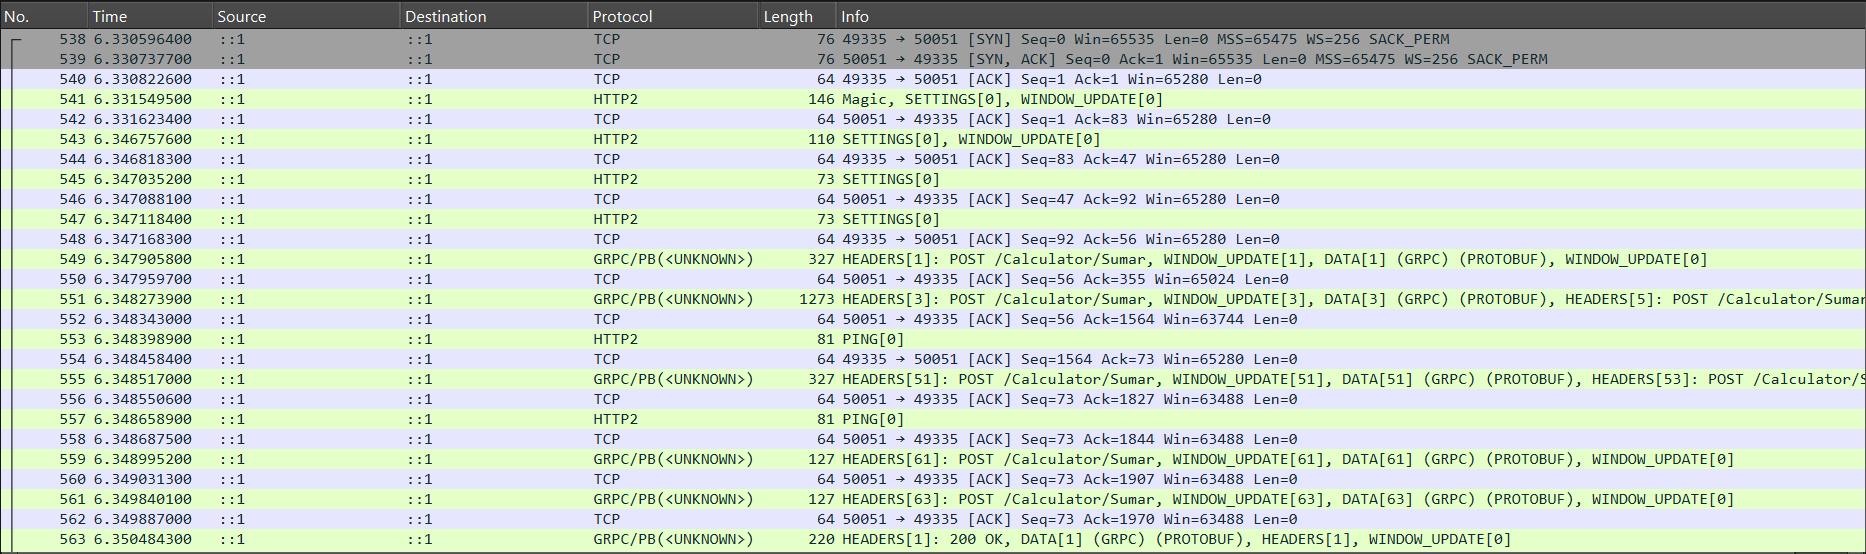
\includegraphics[width=\linewidth]{img/5_a.png}
\caption{Captura Wireshark escenario 1.}
\label{fig:5_a}
\end{figure}

\subsection{Escenario 2: \texttt{delay = 100 \text{ms}}, \texttt{jitter = 0}, \texttt{errores = 0}, \texttt{N = 100} }

En este escenario la comunicación ocurre en un único \textit{socket}, es decir, en una única comunicación TCP, esto se puede verificar observando que existe un único \textit{3-way handshake} al inicio de la conexión tal y como se observa en la Figura \ref{fig:5_b}.

Nuevamente, al igual que en el escenario anterior, se observa el patrón concurrente de las transacciones gracias a multiplexación y a la identificación mediante el \textit{stream} ID. En la Figura \ref{fig:5_b_final} se observa que las respuestas del servidor tienden a estar ordenadas pero no de forma excluyente ---véase tramas 2236 (\texttt{HEADERS [85]}), 2238 (\texttt{HEADERS [89]}) y 2240 (\texttt{HEADERS [87]})---.

\begin{figure}[H]
\centering
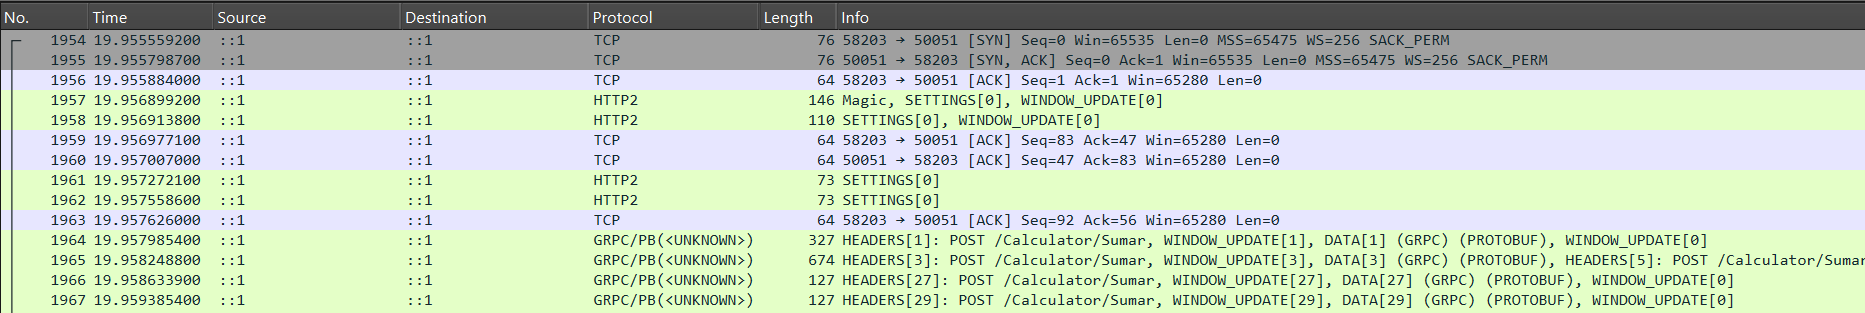
\includegraphics[width=\linewidth]{img/5_b.png}
\caption{Captura Wireshark escenario 2.}
\label{fig:5_b}

\centering
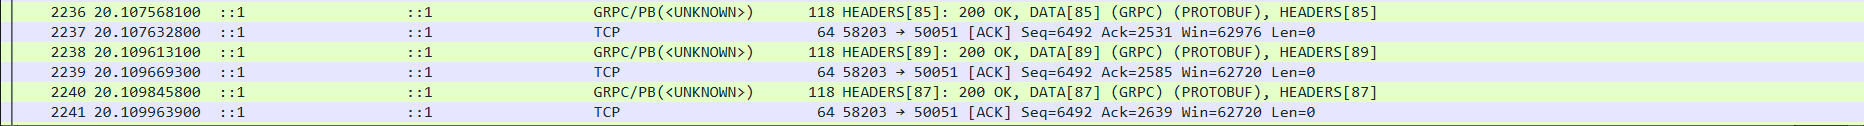
\includegraphics[width=\linewidth]{img/5_b_final.png}
\caption{Captura Wireshark escenario 2 (continuación).}
\label{fig:5_b_final}
\end{figure}

El RTT medio obtenido en esta comunicación es 124.453 ms y su desvío estándar resultó 3.428 ms. El parámetro \texttt{jitter = 0} en el \textit{script} asegura que la red no aumente su variabilidad. Sin embargo, el desvío estándar de unos pocos milisegundos existe por retrasos propios del Sistema Operativo. Nótese que en este escenario, la media del RTT resultó aproximadamente 100 ms mayor que en el escenario anterior.

Para observar los 100 ms en una sola transacción, podemos considerar el primer \textit{stream} ID:
\begin{align*}
\texttt{No.: 1964} &\quad \texttt{Time: 19.957985400} \quad \texttt{Info: HEADERS[1]: POST /Calculator/Sumar (...)} \\
\texttt{No.: 2138} &\quad \texttt{Time: 20.061814900} \quad \texttt{{Info: HEADERS[1]: 200 OK (...)}}
\end{align*}

Computando la diferencia de tiempo entre la solicitud del cliente y la respuesta del servidor, obtenemos un \textit{delay} aproximado de 103 ms.


Al extrapolar el concepto de \textit{delay} a la Internet global, este no se limita solo a la velocidad de transmisión, sino que se manifiesta en cualquier punto donde los datos deban viajar, procesarse o esperar en cola. Percibimos este retraso en múltiples contextos reales de la red, por ejemplo: cuando los paquetes de datos deben recorrer miles de kilómetros de fibra óptica (\textit{propagation delay}), cuando un servidor web remoto debe buscar información pesada en una base de datos (\textit{processing delay}), o cuando la infraestructura de red está saturada por alto tráfico y los paquetes deben esperar su turno en las colas de los \textit{routers} (\textit{queuing delay}), causando lentitud generalizada.

\subsection{Escenario 3: \texttt{delay = 100 \text{ms}}, \texttt{jitter = 100 ms}, \texttt{errores = 0}, \texttt{N = 100} }

El RTT medio obtenido en este escenario es 125.358 ms y su desvío estándar 60.740 ms. El primer valor es correcto y consistente con los escenarios anteriores, en cambio, el segundo, es muy alto (dado por el \texttt{jitter = 100}) lo que significa que existen paquetes que tardaron unos 65 ms y otros más de 180 ms.

En esta situación se observa de forma muy marcada en el desorden en las respuestas del servidor (Figura \ref{fig:5_c}). Podemos resumir el funcionamiento de esta manera:
\begin{itemize}
    \item El cliente envía las solicitudes con un \textit{stream} ID impar de forma secuencial (1, 3, 5, 7, ...)
    \item El servidor recibe las peticiones pero, por culpa del \textit{jitter} introducido, cada respuesta debe esperar un tiempo aleatorio.
    \item La multiplexación permite que el cliente pueda seguir enviando solicitudes sin bloquearse por las demoras del servidor y, a su vez, que el servidor no deba esperar, por ejemplo, que la respuesta No. 5 esté lista para enviar la No. 42.
    \item A pesar del desorden temporal en las respuestas del servidor, el cliente puede identificar qué respuesta corresponde a qué pregunta gracias al \textit{stream} ID.
\end{itemize}

\begin{figure}[H]
\centering
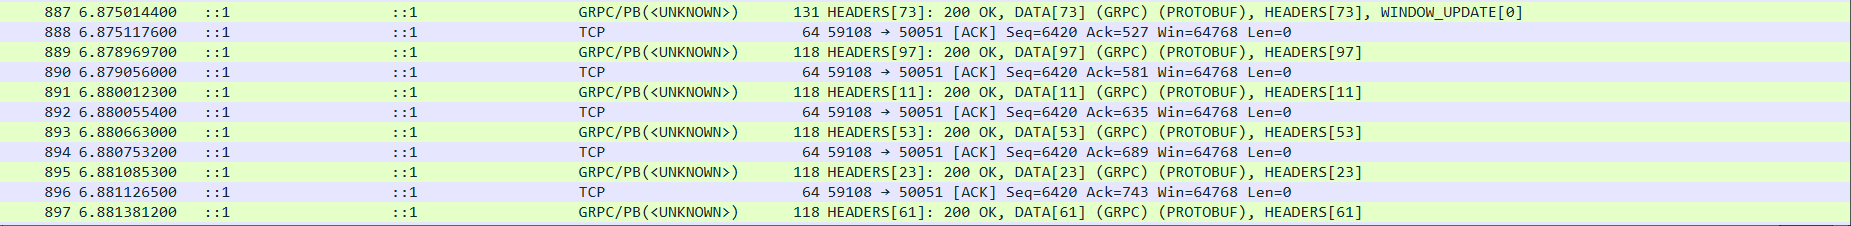
\includegraphics[width=\linewidth]{img/5_c.png}
\caption{Captura Wireshark escenario 3.}
\label{fig:5_c}
\end{figure}


Un efecto análogo en la Internet global, el (\textit{jitter}) puede observar en servicios de \textit{streaming} de video en vivo (Twitch, transmisiones deportivas, etc.). En estos contextos, si los paquetes de datos atraviesan rutas dinámicas o sufren congestiones variables, llegarán al destino con retardos impredecibles y desordenados. Al no disponer de los paquetes en el momento exacto que deben reproducirse, se generan congelamientos en el video o cortes e interrupciones en el audio. Para mitigar este fenómeno, las aplicaciones de \textit{streaming} emplean búferes de \textit{jitter} (\textit{jitter buffers}), los cuales retienen intencionalmente la reproducción unos milisegundos para absorber la variabilidad, dar tiempo a que lleguen los paquetes atrasados y reordenarlos antes de presentarlos al usuario.


\subsection{Escenario 4: \texttt{delay = 100 \text{ms}}, \texttt{jitter = 100 ms}, \texttt{errores = 20\%}, \texttt{N = 100} }
En este escenario mantenemos los valores del anterior pero agregamos un porcentaje de error. Se obtiene un RTT medio de 116.106 ms y un desvío de 57.593 ms y 26 errores. Es interesante destacar que, como el código \texttt{server\_delay.py} evalúa la probabilidad de error y luego ejecuta el delay (\textit{Fast-fail}), todas las peticiones con error tienen un RTT mucho menor al del promedio (del orden de los 20 ms).

En la consola, al ejecutar el código, se puede observar que el estado es \texttt{status = INTERNAL}, indicando que el mensaje alcanzó el destino pero el servidor encontró una excepción interna al intentar procesar la operación.

Al inspeccionar los paquetes de respuesta enviados por el servidor en \textit{Wireshark}, se puede determinar el resultado analizando el campo \texttt{grpc-status} que viaja en los \textit{Trailers} de HTTP/2 (Figuras \ref{fig:grpc_ok} y \ref{fig:grpc_error}):
\begin{itemize}
    \item Los paquetes sin error devuelven el código \texttt{grpc-status: 0 (OK)} .
    \item Los paquetes con error devuelven el código \texttt{grpc-status: 13 (INTERNAL)}. Además, se observa que estos paquetes omiten por completo la trama \texttt{DATA} y envían un único bloque \texttt{HEADERS}
\end{itemize}

\begin{figure}[H]
\centering
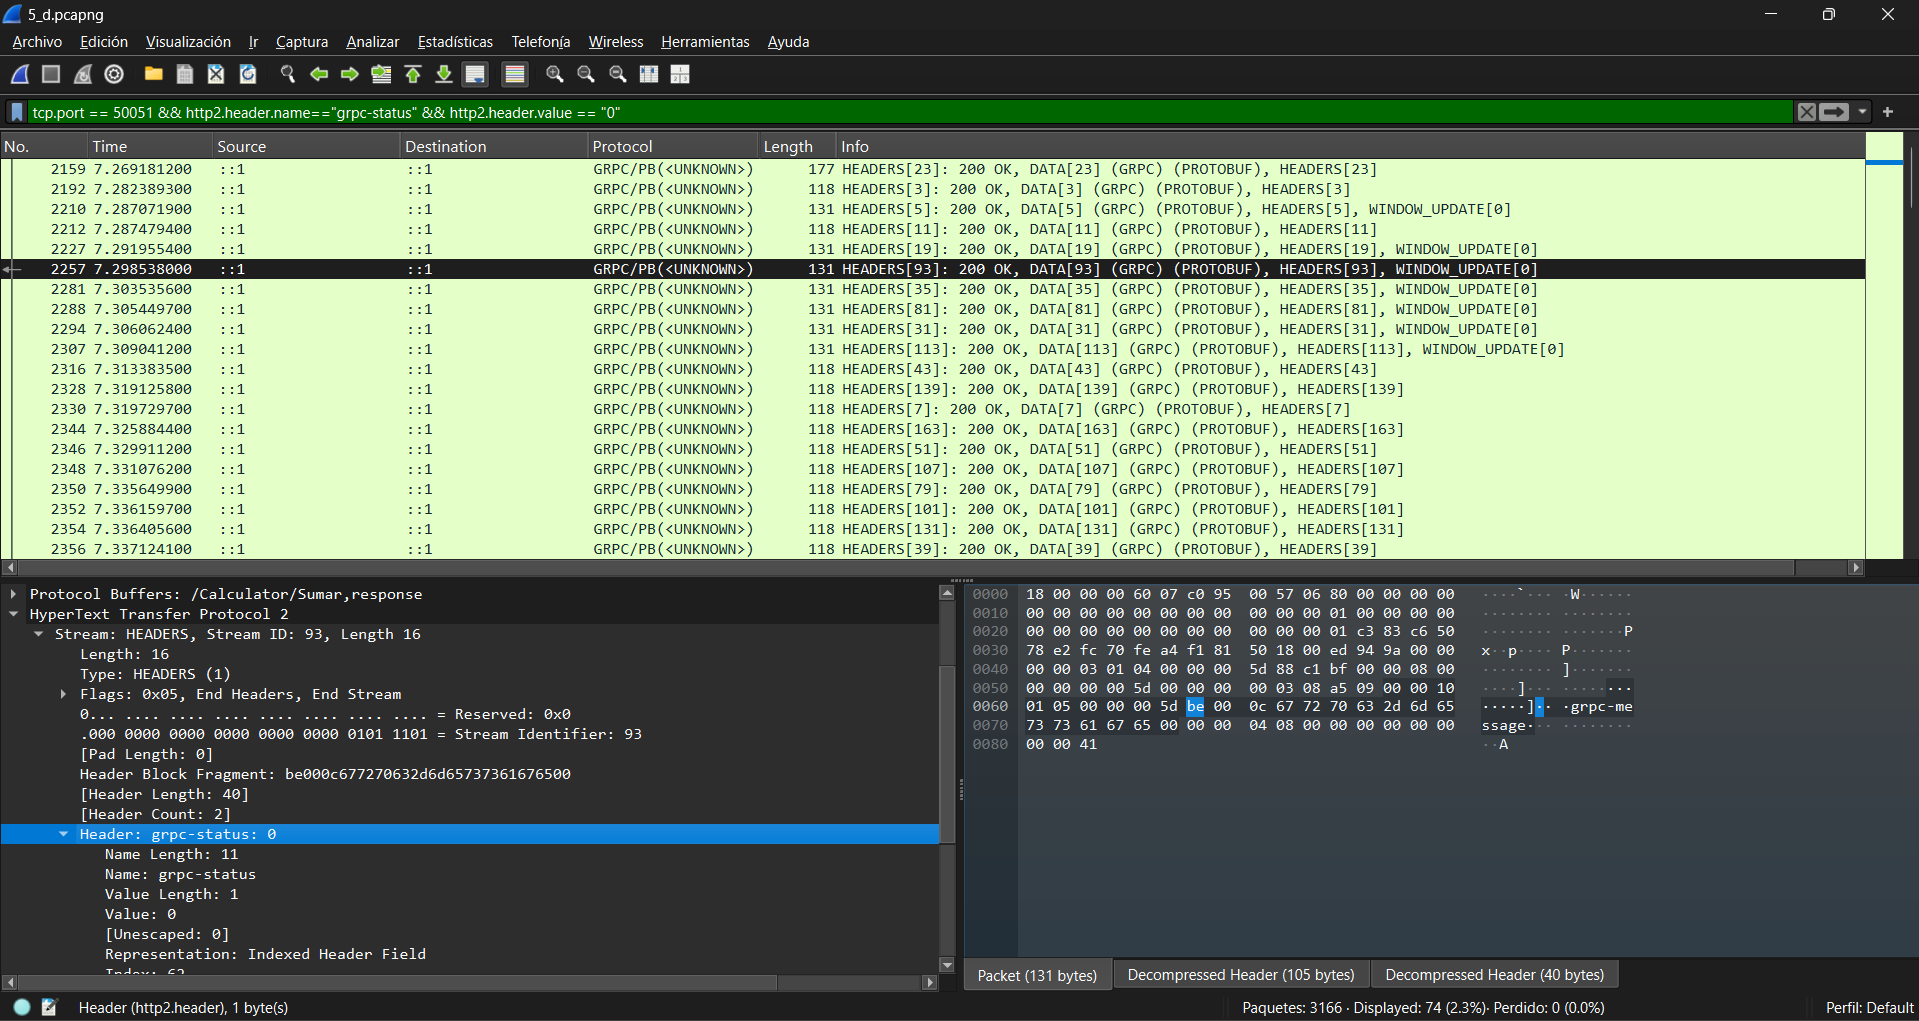
\includegraphics[width=\linewidth]{img/grpc_status_ok.png}
\caption{grpc-status: 0.}
\label{fig:grpc_ok}

\centering
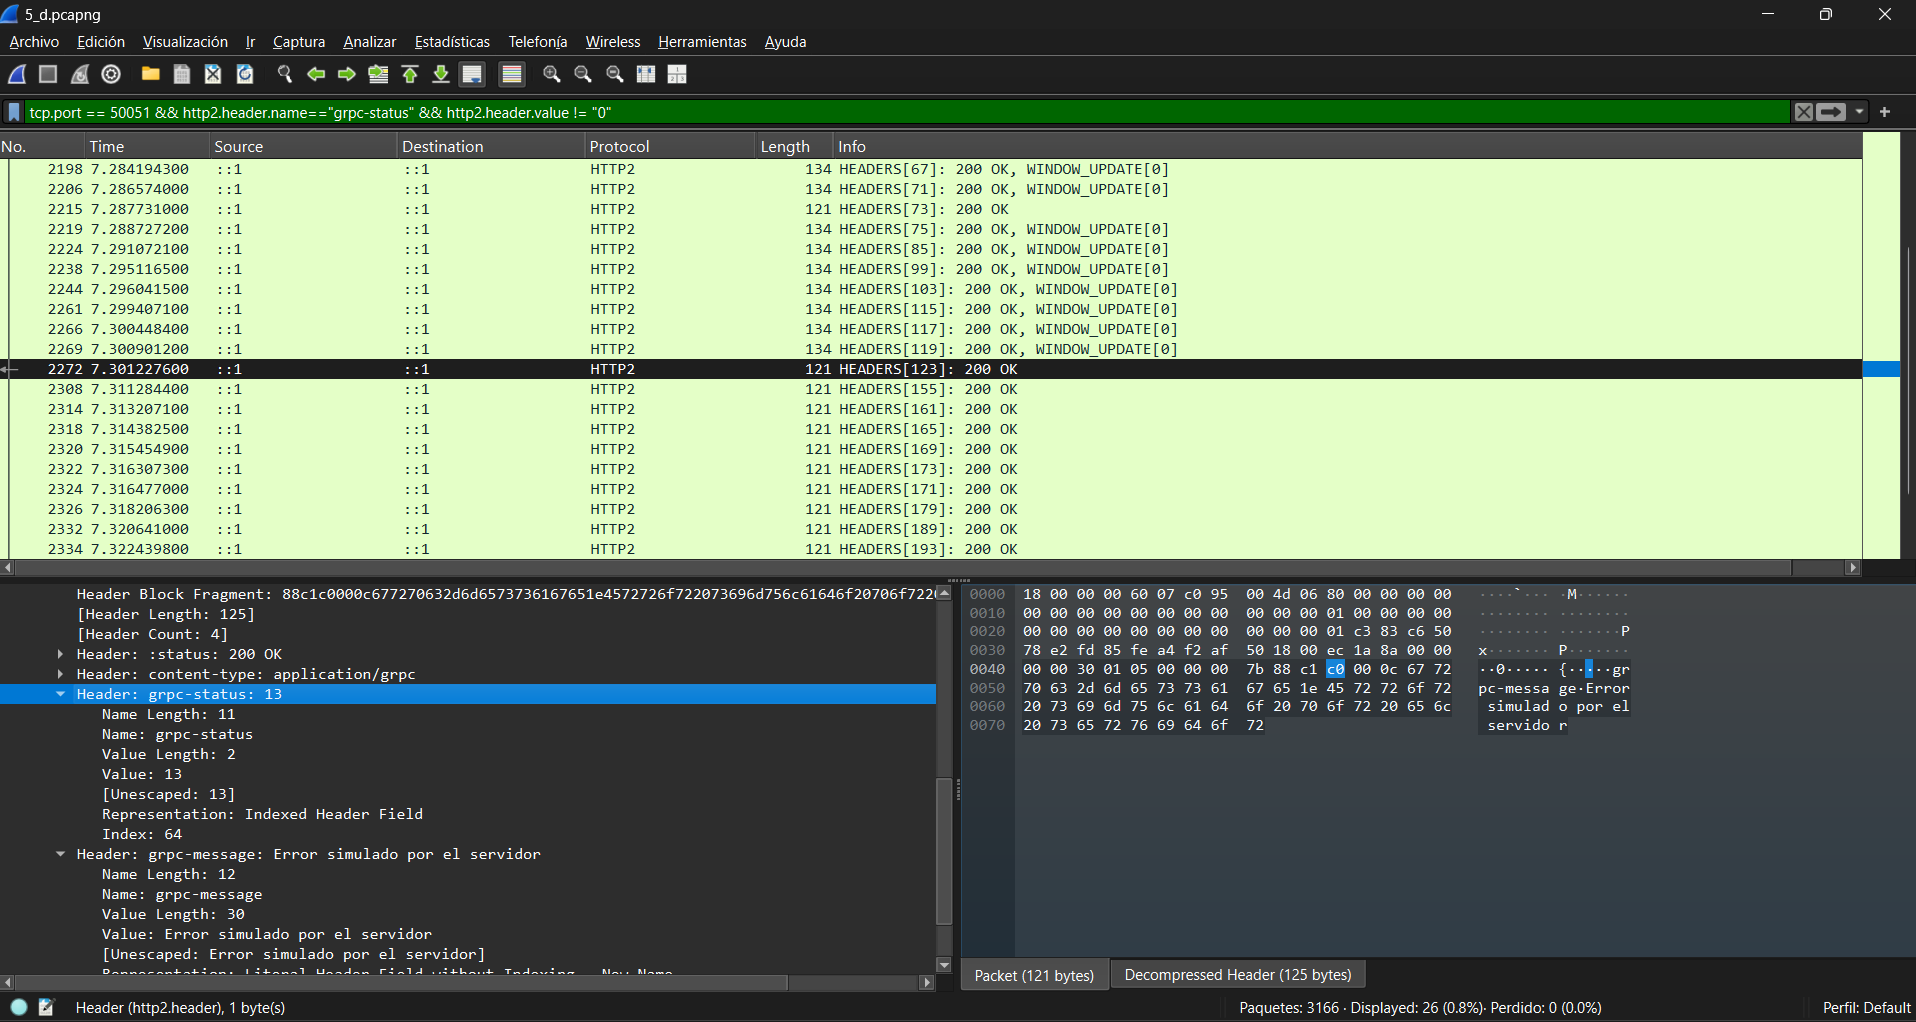
\includegraphics[width=\linewidth]{img/grpc_status_error.png}
\caption{grpc-status: 13.}
\label{fig:grpc_error}
\end{figure}       

gRPC contiene en su estándar 16 códigos de error para múltiples situaciones, las más comunes son:
\begin{itemize}
    \item \texttt{DEADLINE\_EXCEEDED}: código 4, cuando expira el tiempo máximo de espera.
    \item \texttt{UNAVAILABLE}: código 14, servidor inalcanzable por fallas de red.
    \item \texttt{UNIMPLEMENTED}: código 12, método inexistente.
    \item \texttt{UNAUTHENTICATED}: código 16, credenciales inválidas.
\end{itemize}

Es importante destacar que un error en el servicio gRPC no implica un error en HTTP/2. Pues el segundo únicamente tiene la responsabilidad de entregar el paquete con éxito. En consecuencia, se sigue observando un estado HTTP/2 de ``\texttt{200 OK}'' con la diferencia de que aquellos con error no tendrán el frame \texttt{DATA} (ya que gRPC la omite). Este comportamiento se puede observar en la Figura \ref{fig:rta_http2}, en donde el \texttt{HEADERS[23]} (exitoso) contiene el frame \texttt{DATA} y, en cambio, el \texttt{HEADERS[25]} (erróneo) lo omite.


\begin{figure}[H]
\centering
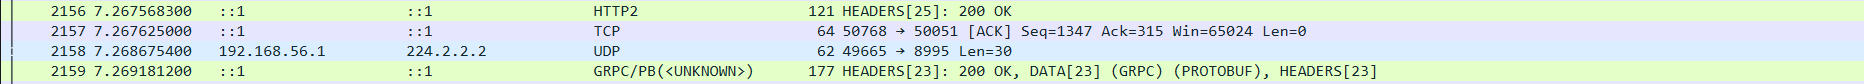
\includegraphics[width=\linewidth]{img/5_c_http.png}
\caption{Repuesta HTTP/2}
\label{fig:rta_http2}
\end{figure}   


\section{Conclusiones}

A lo largo de este trabajo práctico, se logró contrastar la teoría subyacente a gRPC, HTTP/2 y TCP con el comportamiento empírico observado en la red mediante Wireshark. El análisis del tráfico permitió validar el funcionamiento de la multiplexación de HTTP/2, permitiendo la transmisión concurrente de múltiples peticiones mediante \textit{Stream IDs} independientes sobre un único \textit{socket} TCP.

Asimismo, la simulación de distintos escenarios demostró el impacto real de parámetros como el retardo y la fluctuación (\textit{jitter}). Se evidenció empíricamente que, frente a latencias variables, las respuestas pierden su orden secuencial inicial, un fenómeno que en la Internet global afecta críticamente a servicios en tiempo real. 

Finalmente, la inyección de fallos permitió comprender la separación de responsabilidades entre capas: un error lógico de aplicación (gRPC status 13) es manejado de forma independiente al transporte, manteniendo intacto el estado de éxito (\texttt{200 OK}) en la capa HTTP/2. En conjunto, estas observaciones demuestran la eficiencia, concurrencia y robustez de gRPC para el desarrollo de sistemas distribuidos modernos.

\begin{thebibliography}{9}

\bibitem{ref1}
J. F. Kurose y K. W. Ross,
\textit{Redes de computadoras: Un enfoque descendente},
7.\ ed.,
Pearson Educación, Madrid, 2017.

\bibitem{ref2}
gRPC Authors,
\textit{gRPC Documentation},
disponible en: \texttt{https://grpc.io/docs/},
consultado en abril de 2026.

\bibitem{ref3}
The Linux Foundation,
\textit{Protocol Buffers Documentation},
disponible en: \texttt{https://protobuf.dev/},
consultado en abril de 2026.

\bibitem{ref4}
Internet Engineering Task Force (IETF),
\textit{Hypertext Transfer Protocol Version 2 (HTTP/2)},
RFC 9113, junio de 2022.
Disponible en: \texttt{https://www.rfc-editor.org/rfc/rfc9113.html},
consultado en abril de 2026. 

\bibitem{ref6}
Wireshark Foundation,
\textit{Wireshark User's Guide},
disponible en: \texttt{https://www.wireshark.org/docs/},
consultado en abril de 2026.

\bibitem{ref7}
Python Software Foundation,
\textit{Python 3 Documentation},
disponible en: \texttt{https://docs.python.org/3/},
consultado en abril de 2026.

\bibitem{ref8}
Internet Assigned Numbers Authority (IANA),
\textit{Service Name and Transport Protocol Port Number Registry},
disponible en: \texttt{https://www.iana.org/assignments/service-names-port-numbers/},
consultado en abril de 2026.

\end{thebibliography}

\end{document}